\documentclass[aspectratio=169,11pt]{beamer}

% ---------------------------------------------------------------------------
% Quantathon CR 2026 -- Challenge 3
% Charla de 10 minutos (acompana al poster): Fermi-Hubbard en escalera 3x2
% Misma paleta que presentacion_fermi_hubbard{,_resultados}.tex.
% Compilar desde Informe_tecnico/: las figuras se leen de ../fermi_hubbard_*.png
% Tiempos sugeridos en los comentarios de cada seccion (total ~10 min).
% ---------------------------------------------------------------------------

\usetheme{Madrid}
\usecolortheme{default}
\setbeamertemplate{navigation symbols}{}
\setbeamertemplate{footline}[frame number]

\usepackage[utf8]{inputenc}
\usepackage[T1]{fontenc}
\usepackage{amsmath,amssymb}
\usepackage{braket}
\usepackage{booktabs}
\usepackage{graphicx}
\usepackage{tikz}
\usetikzlibrary{arrows.meta,positioning,calc}

\definecolor{qDeep}{RGB}{35,32,90}
\definecolor{qMid}{RGB}{75,55,160}
\definecolor{qAccent}{RGB}{0,150,170}
\definecolor{qWarn}{RGB}{190,60,50}
\definecolor{qGray}{RGB}{90,90,95}

\setbeamercolor{structure}{fg=qMid}
\setbeamercolor{title}{fg=white,bg=qDeep}
\setbeamercolor{frametitle}{fg=white,bg=qDeep}
\setbeamercolor{palette primary}{fg=white,bg=qDeep}
\setbeamercolor{palette secondary}{fg=white,bg=qMid}
\setbeamercolor{palette tertiary}{fg=white,bg=qDeep}
\setbeamercolor{block title}{fg=white,bg=qMid}
\setbeamercolor{block body}{bg=qMid!8}
\setbeamercolor{block title alerted}{fg=white,bg=qWarn}
\setbeamercolor{block body alerted}{bg=qWarn!8}
\setbeamercolor{item}{fg=qAccent}
\setbeamerfont{frametitle}{series=\bfseries}

\newcommand{\good}[1]{\textcolor{qAccent}{\textbf{#1}}}
\newcommand{\warn}[1]{\textcolor{qWarn}{\textbf{#1}}}

\title[Fermi-Hubbard en escalera $3\times2$]{Modelo de Fermi-Hubbard en una escalera $3\times2$}
\subtitle{¿Qué tan lejos llegan los métodos cuánticos frente a la solución exacta?}
\author{Quantathon CR 2026 -- QWorld Hackathon, Challenge 3}
\date{}

\begin{document}

% ============================================================= 0:00
\begin{frame}
  \titlepage
\end{frame}

% ============================================================= 0:15 -- 1:30
\begin{frame}{El problema}
  \begin{columns}[T]
    \begin{column}{0.56\textwidth}
      \[
        H = -t\!\sum_{\langle ij\rangle,\sigma}\!\left(c^\dagger_{i\sigma}c_{j\sigma}+\text{h.c.}\right)
            + U\sum_i n_{i\uparrow}n_{i\downarrow} - \mu\sum_{i\sigma} n_{i\sigma}
      \]
      \begin{itemize}
        \item Escalera $3\times2$: piernas periódicas, peldaños abiertos.
        \item 6 sitios $\Rightarrow$ \textbf{12 qubits} (Jordan-Wigner, bloque $\uparrow$ luego
          $\downarrow$).
        \item Llenado medio: $N_\uparrow=N_\downarrow=3$, $\mu=U/2$; barremos $U/t$.
        \item \warn{Escalera de 2 piernas: crossover, no transición de fase} -- no hay un $U_c$.
      \end{itemize}
    \end{column}
    \begin{column}{0.42\textwidth}
      \centering
      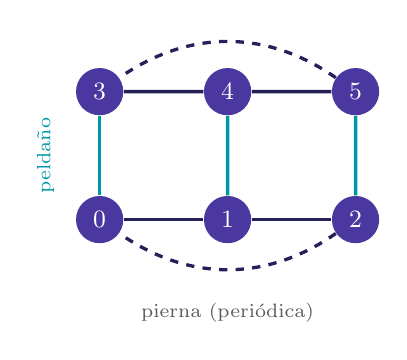
\begin{tikzpicture}[scale=1.25,
          site/.style={circle,fill=qMid,text=white,minimum size=6mm,inner sep=0pt,font=\small}]
        \foreach \x in {0,1,2} {
          \node[site] (a\x) at (\x*1.3,0) {\the\numexpr\x\relax};
          \node[site] (b\x) at (\x*1.3,1.3) {\the\numexpr\x+3\relax};
          \draw[qAccent,very thick] (a\x) -- (b\x);
        }
        \draw[qDeep,very thick] (a0)--(a1)--(a2); \draw[qDeep,very thick] (b0)--(b1)--(b2);
        \draw[qDeep,very thick,dashed] (a2) to[bend left=35] (a0);
        \draw[qDeep,very thick,dashed] (b2) to[bend right=35] (b0);
        \node[font=\scriptsize,qGray] at (1.3,-0.95) {pierna (periódica)};
        \node[font=\scriptsize,qAccent,rotate=90] at (-0.55,0.65) {peldaño};
      \end{tikzpicture}
      \vspace{0.5em}

      \small Plan: \textbf{ED} (exacto) como referencia, contra \textbf{Trotter} y
      \textbf{VQE} en Qiskit.
    \end{column}
  \end{columns}
\end{frame}

% ============================================================= 1:30 -- 2:00
\begin{frame}{Por qué $3\times2$ (y no $4\times2$ como se planeó)}
  \begin{columns}[T]
    \begin{column}{0.5\textwidth}
      \begin{alertblock}{VQE a 16 qubits no convergió}
        Ni siquiera en $U=0$: $E_{\text{VQE}}=-5.28$ vs.\ $E_{\text{exacto}}=-12.00$.
      \end{alertblock}
      \begin{block}{A 12 qubits}
        $\sim$0.04\,s por circuito (vs.\ 0.3--0.7\,s): permite un ángulo libre por enlace y
        varios reinicios de COBYLA. Se usó $3\times2$ en \emph{todo} el proyecto.
      \end{block}
    \end{column}
    \begin{column}{0.48\textwidth}
      \textbf{Costo estructural:} un anillo de 3 sitios \warn{no es bipartito} -- dos
      enlaces cualesquiera comparten un vértice.
      \vspace{0.5em}

      $\Rightarrow$ el paso de Trotter necesita \textbf{9 capas} de compuertas que conmutan,
      no 7.
      \vspace{0.5em}

      \small 10 de los 18 términos de hopping llevan cadenas de $Z$ (longitud 1 o 2): el costo
      de Jordan-Wigner en 2D.
    \end{column}
  \end{columns}
\end{frame}

% ============================================================= 2:00 -- 3:30
\begin{frame}{A · Diagonalización exacta: el crossover}
  \centering
  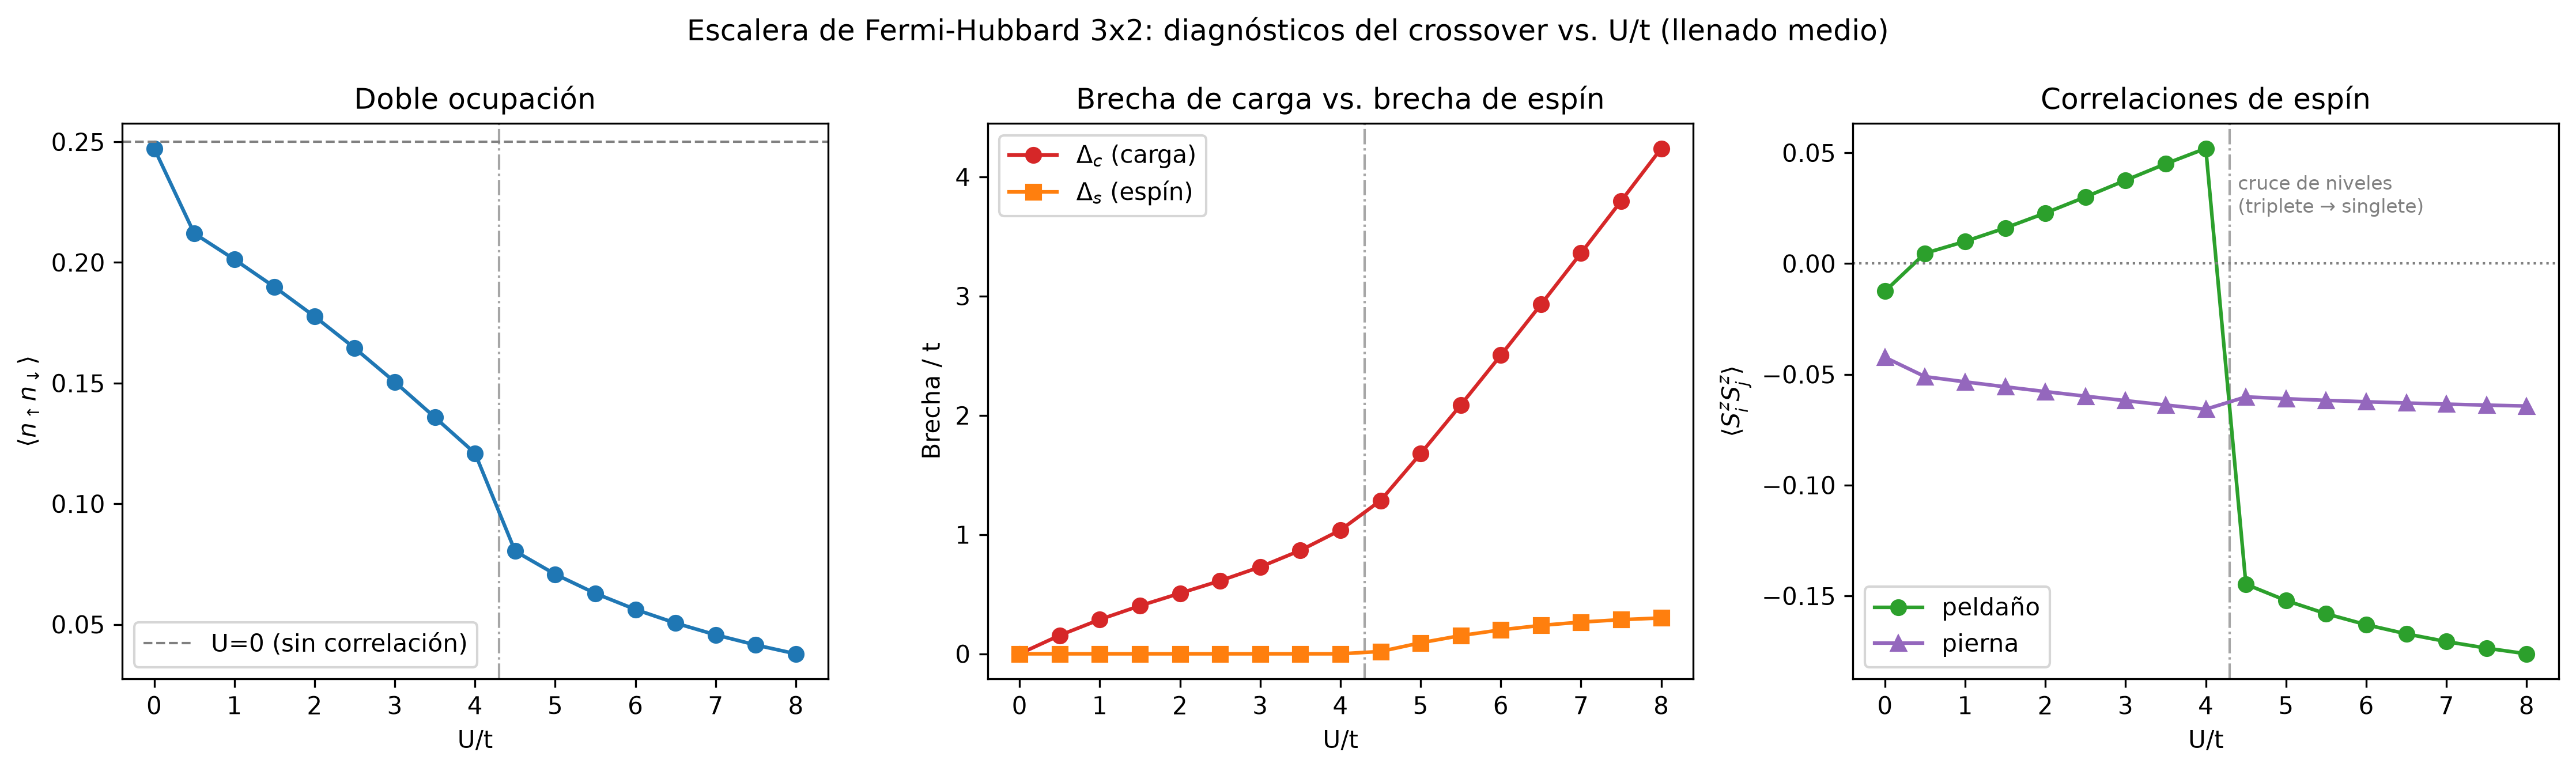
\includegraphics[width=\textwidth]{../fermi_hubbard_2d_phase_diagram.png}
  \vspace{0.2em}

  \small Sector de llenado medio: dimensión 400 -- 17 valores de $U/t$ en $<$1\,s.
  \quad \good{$\Delta_c$: de 0 a $\sim$4.2}, \quad doble ocupación: de $\approx0.25$ a 0.04.
\end{frame}

\begin{frame}{A · Un cruce de niveles de tamaño finito en $U/t\approx4.3$}
  \begin{columns}[T]
    \begin{column}{0.48\textwidth}
      \begin{block}{$U/t\lesssim4.3$: triplete ($S=1$)}
        $\Delta_s=0$ exactamente; peldaños débilmente \emph{ferromagnéticos} ($+0.05$).
      \end{block}
    \end{column}
    \begin{column}{0.48\textwidth}
      \begin{block}{$U/t\gtrsim4.3$: singlete de peldaño}
        $\Delta_s$ se abre (0.09\,$\to$\,0.30); peldaños antiferromagnéticos ($-0.18$).
      \end{block}
    \end{column}
  \end{columns}
  \vspace{0.6em}
  \begin{itemize}
    \item El cruce aparece en \textbf{todos} los observables: salto en el peldaño, quiebre en la
      doble ocupación ($0.121\to0.071$), $\Delta_s$ se enciende.
    \item \textbf{Origen:} niveles de una partícula $\{-3,-1,0,0,2,2\}$ -- a llenado medio el
      nivel $0$ degenerado queda \warn{semi-lleno} (capa abierta) y los espines se alinean
      (tipo regla de Hund).
    \item Solo por encima de $U/t\approx4.3$ vemos la física de escalera esperada.
      Verificado con las energías de los sectores $S_z=0,1,2$.
  \end{itemize}
\end{frame}

% ============================================================= 3:30 -- 6:00
\begin{frame}{B · Trotter: \emph{quench} de decaimiento de doblones}
  \begin{columns}[T]
    \begin{column}{0.55\textwidth}
      \begin{itemize}
        \item \textbf{Estado inicial:} pierna $y{=}0$ con todos sus sitios doblemente
          ocupados, pierna $y{=}1$ vacía (doble ocupación $=0.5$).
        \item Evolucionamos con $U/t\in\{1,4,8\}$ fijo, $T_{\max}=5$, 50 pasos.
        \item Circuito hecho a mano: hopping $=e^{i\theta XX_{\text{str}}}e^{i\theta YY_{\text{str}}}$
          (factorización \emph{exacta}), interacción $=e^{-i\frac{U\Delta t}{4}Z_\uparrow Z_\downarrow}$.
        \item Qiskit Aer, 2000 shots; referencia exacta con \texttt{expm\_multiply}.
      \end{itemize}
    \end{column}
    \begin{column}{0.42\textwidth}
      \begin{block}{¿Por qué este experimento?}
        Es el protocolo de átomos fríos (Strohmaier et al., 2010): un doblón que decae
        libera energía $U$. Si $U\gg t$, no tiene adónde ir.
      \end{block}
    \end{column}
  \end{columns}
\end{frame}

\begin{frame}{B · Resultado: $U/t=1$ vs.\ $U/t=8$}
  \centering
  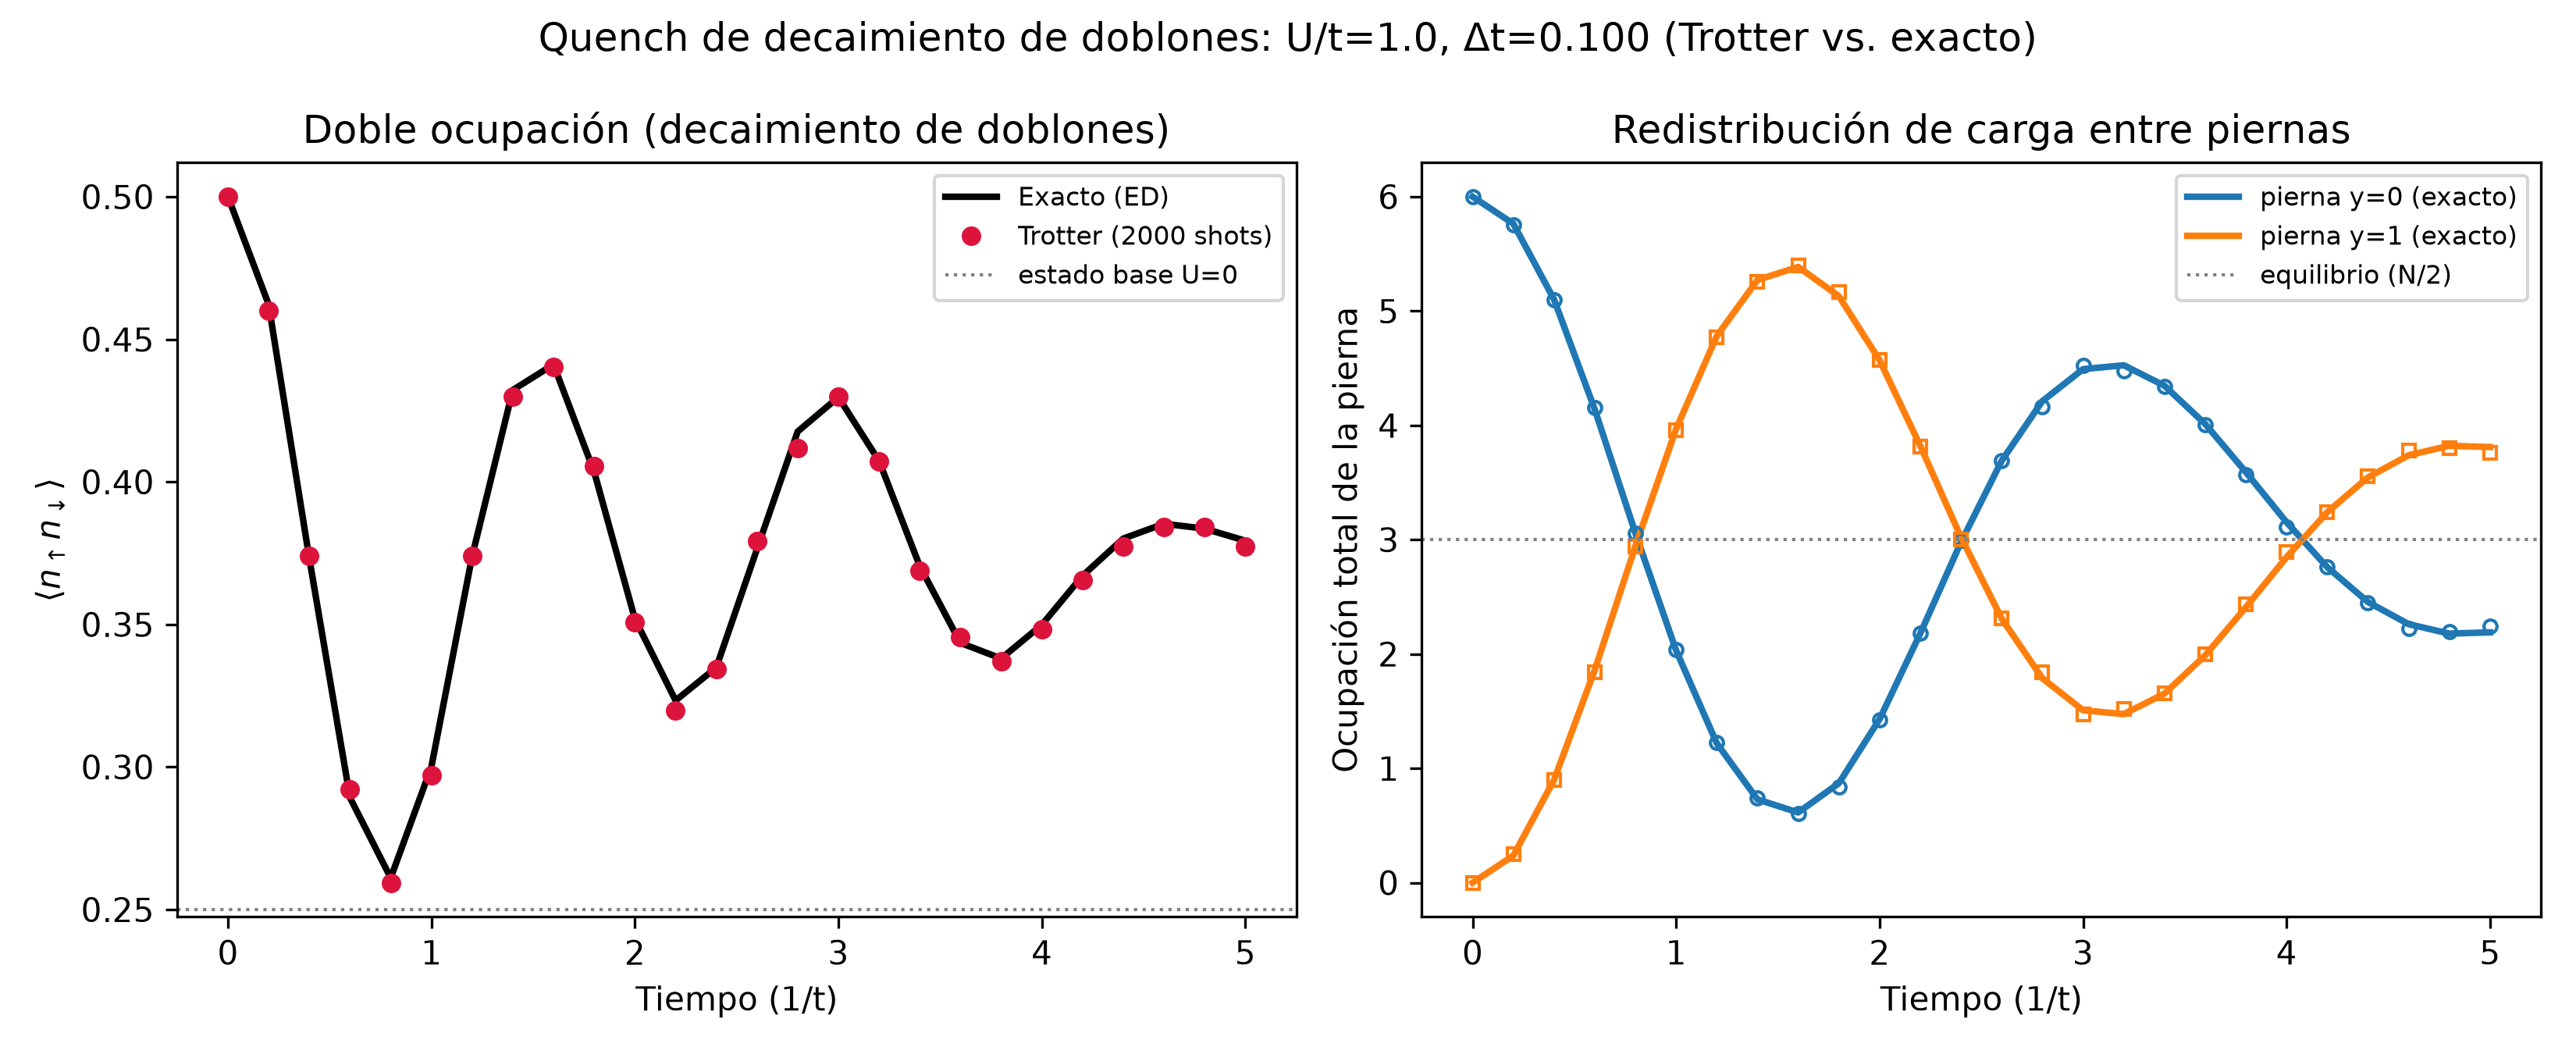
\includegraphics[width=0.49\textwidth]{../fermi_hubbard_quench_U1.0_trotter_vs_exact.png}\hfill
  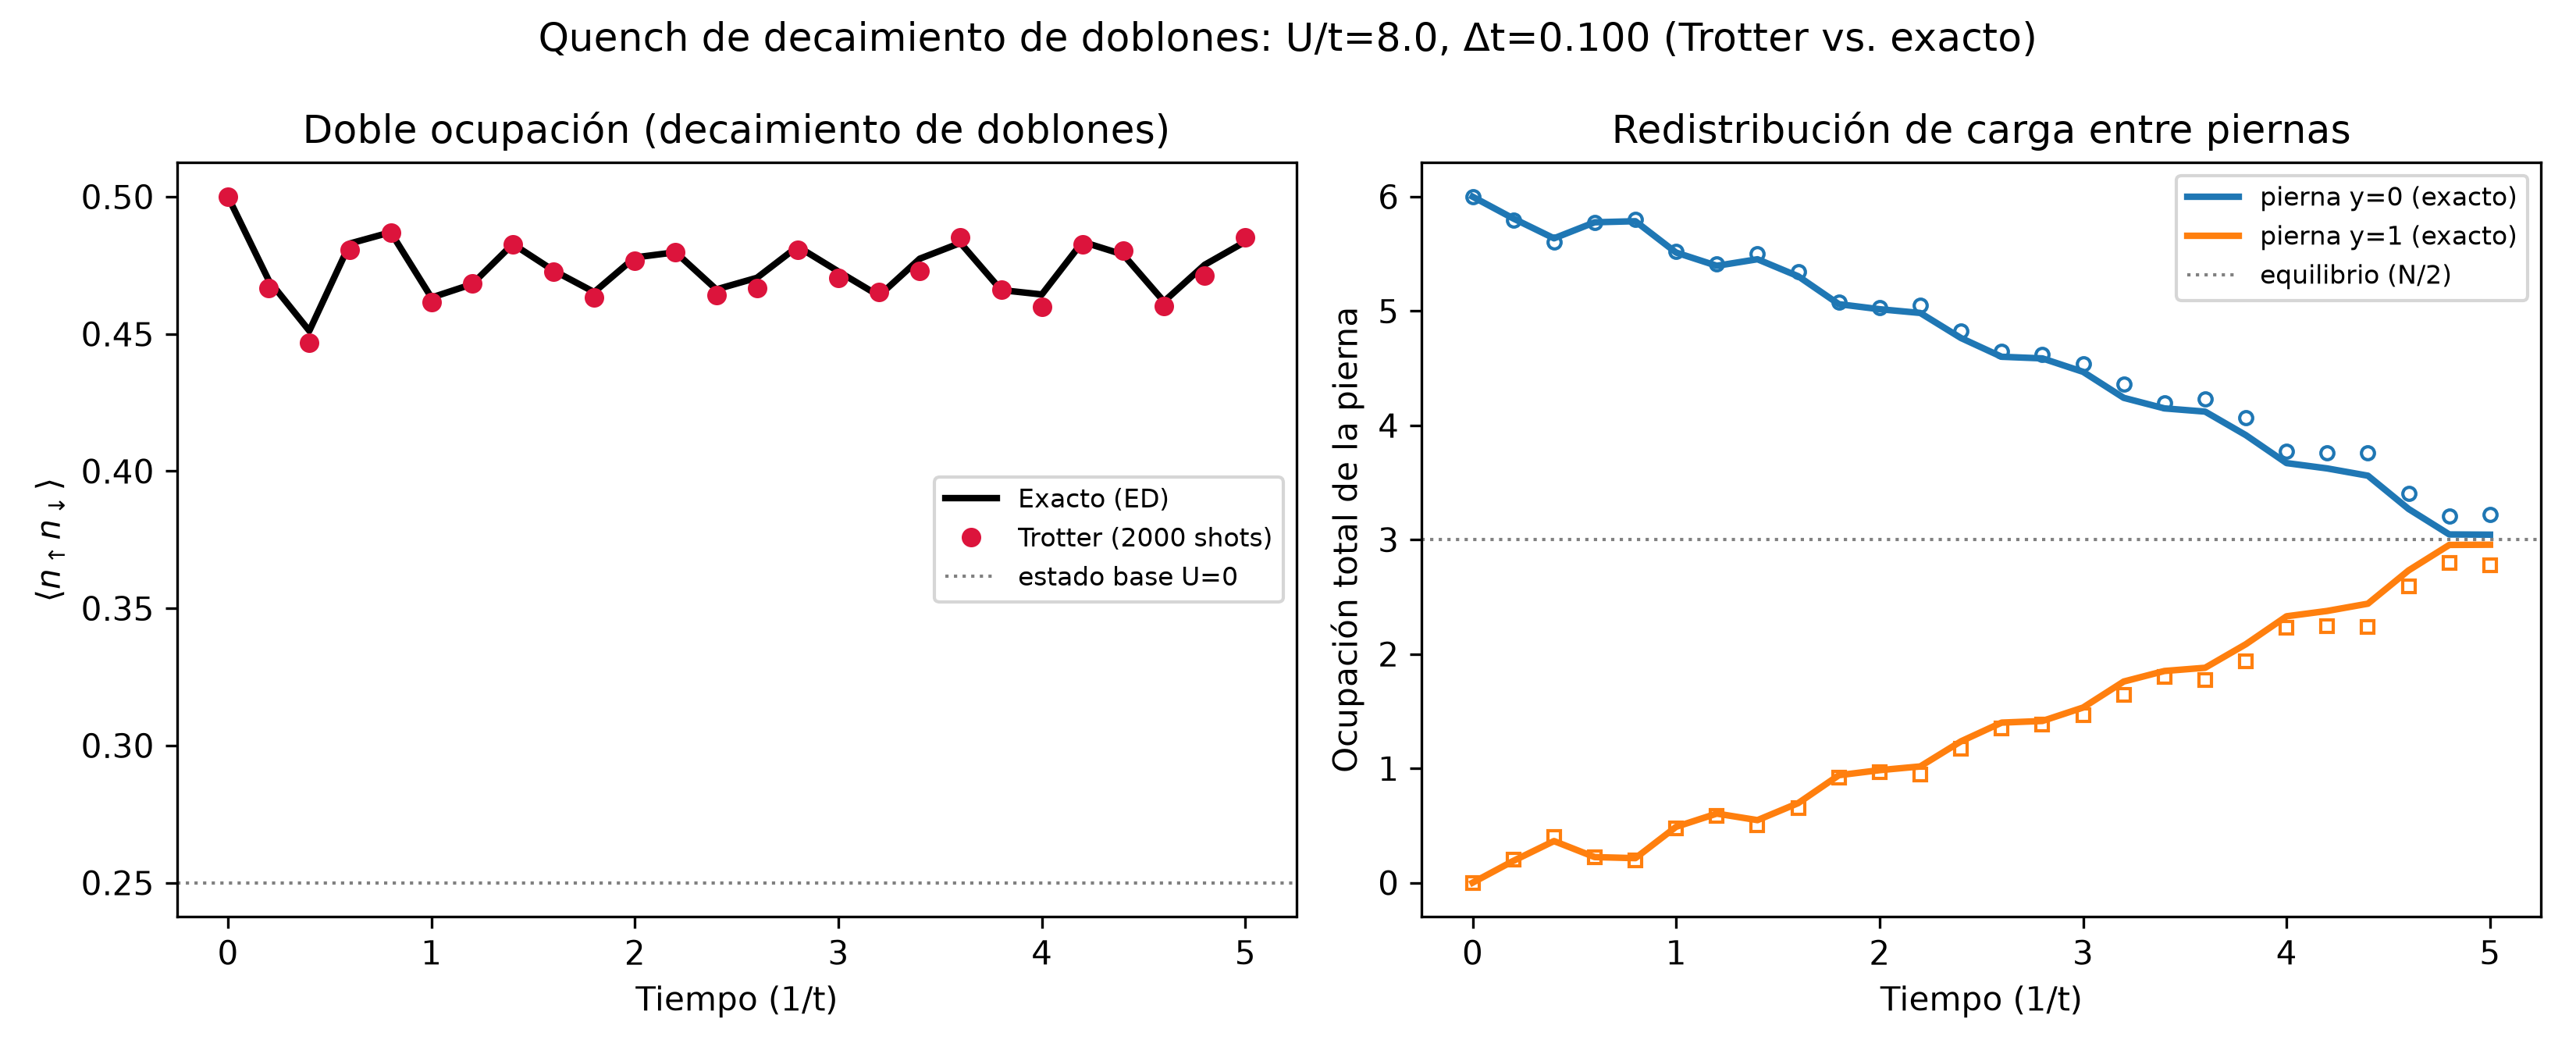
\includegraphics[width=0.49\textwidth]{../fermi_hubbard_quench_U8.0_trotter_vs_exact.png}
  \vspace{0.4em}
  \begin{itemize}
    \item \textbf{$U/t=1$:} los doblones decaen ($0.5\to\sim0.26$) y oscilan entre piernas.
    \item \textbf{$U/t=8$:} \good{decaimiento suprimido} (se queda en 0.46--0.50), aunque la carga
      sí se sigue moviendo.
    \item \good{Trotter vs.\ exacto: diferencia de $\sim$0.001--0.005}, dentro del ruido de shots.
  \end{itemize}
\end{frame}

% ============================================================= 6:00 -- 7:15
\begin{frame}{C · Error de Trotter: medido, no supuesto}
  \begin{columns}[T]
    \begin{column}{0.52\textwidth}
      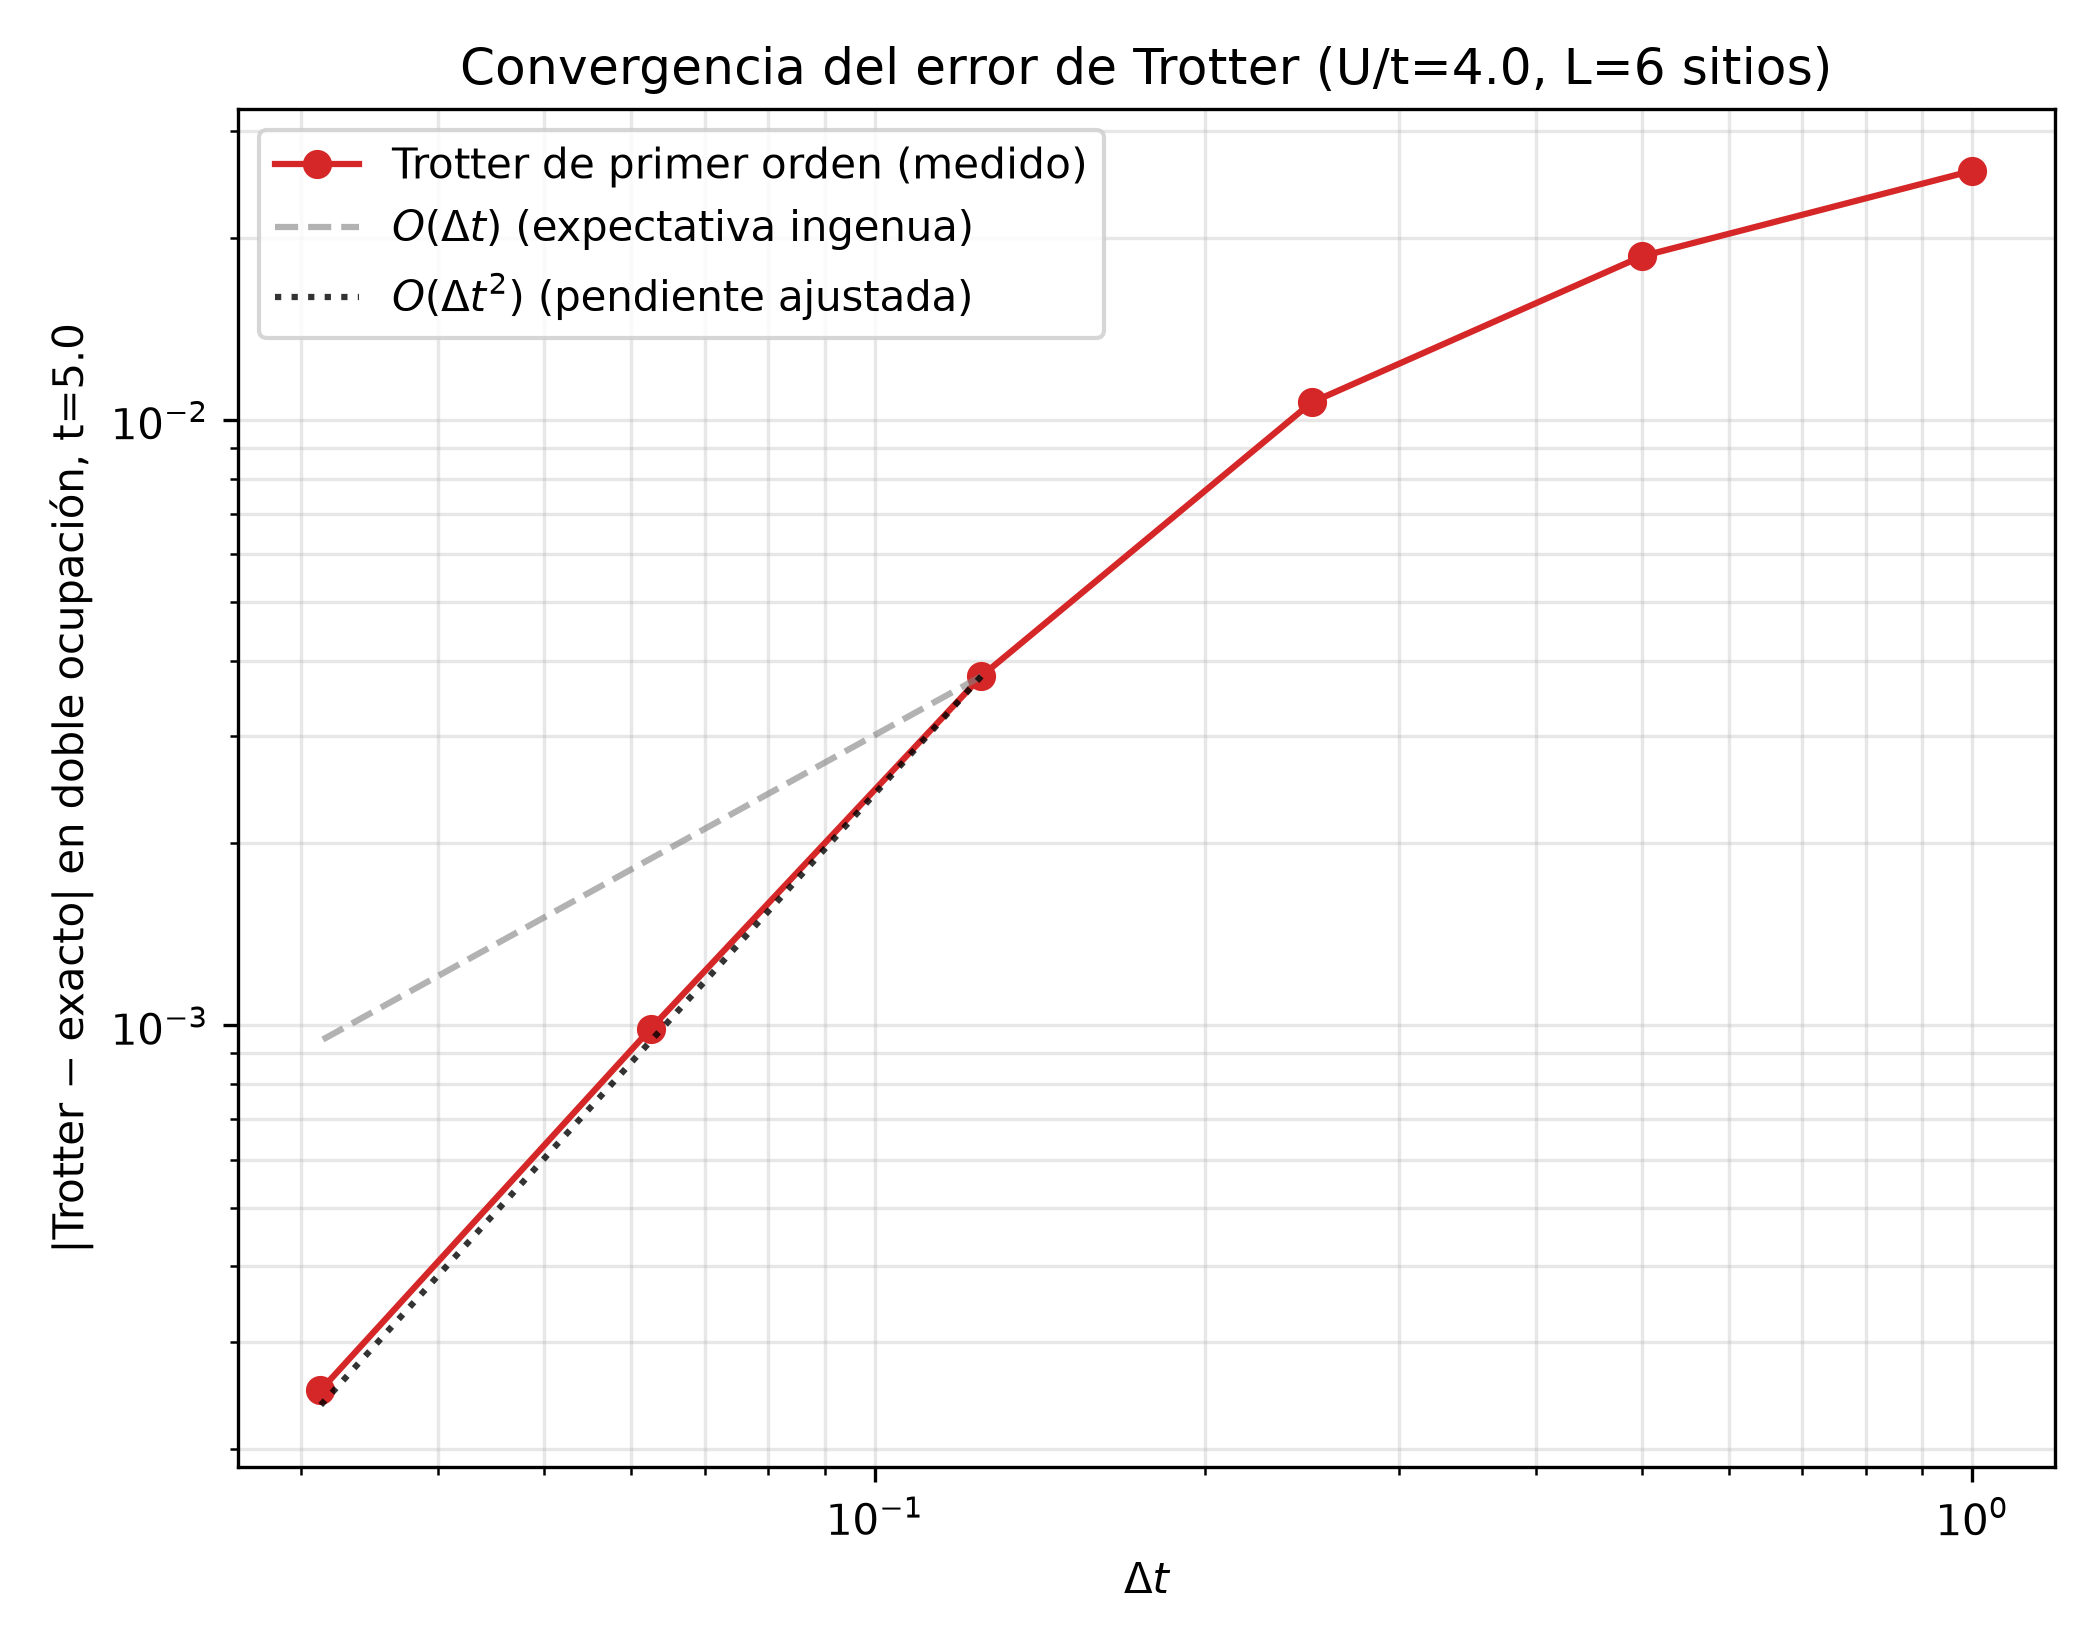
\includegraphics[width=\textwidth]{../fermi_hubbard_trotter_error_convergence.png}
    \end{column}
    \begin{column}{0.46\textwidth}
      \begin{itemize}
        \item $U/t=4$ (el caso más difícil), evaluación exacta sin shots.
        \item $n_{\text{steps}}=5\to160$: error de $0.026$ a $0.00025$.
      \end{itemize}
      \begin{alertblock}{Pendiente asintótica: $\mathbf{1.96}$}
        Más rápida que el $O(\Delta t)$ esperado para primer orden. Se reprodujo en la red
        $4\times2$ original (\textbf{1.98}, con 7 capas): no es casualidad.
      \end{alertblock}
    \end{column}
  \end{columns}
\end{frame}

% ============================================================= 7:15 -- 8:45
\begin{frame}{D · VQE con ansatz Hamiltoniano-Variacional}
  \begin{columns}[T]
    \begin{column}{0.56\textwidth}
      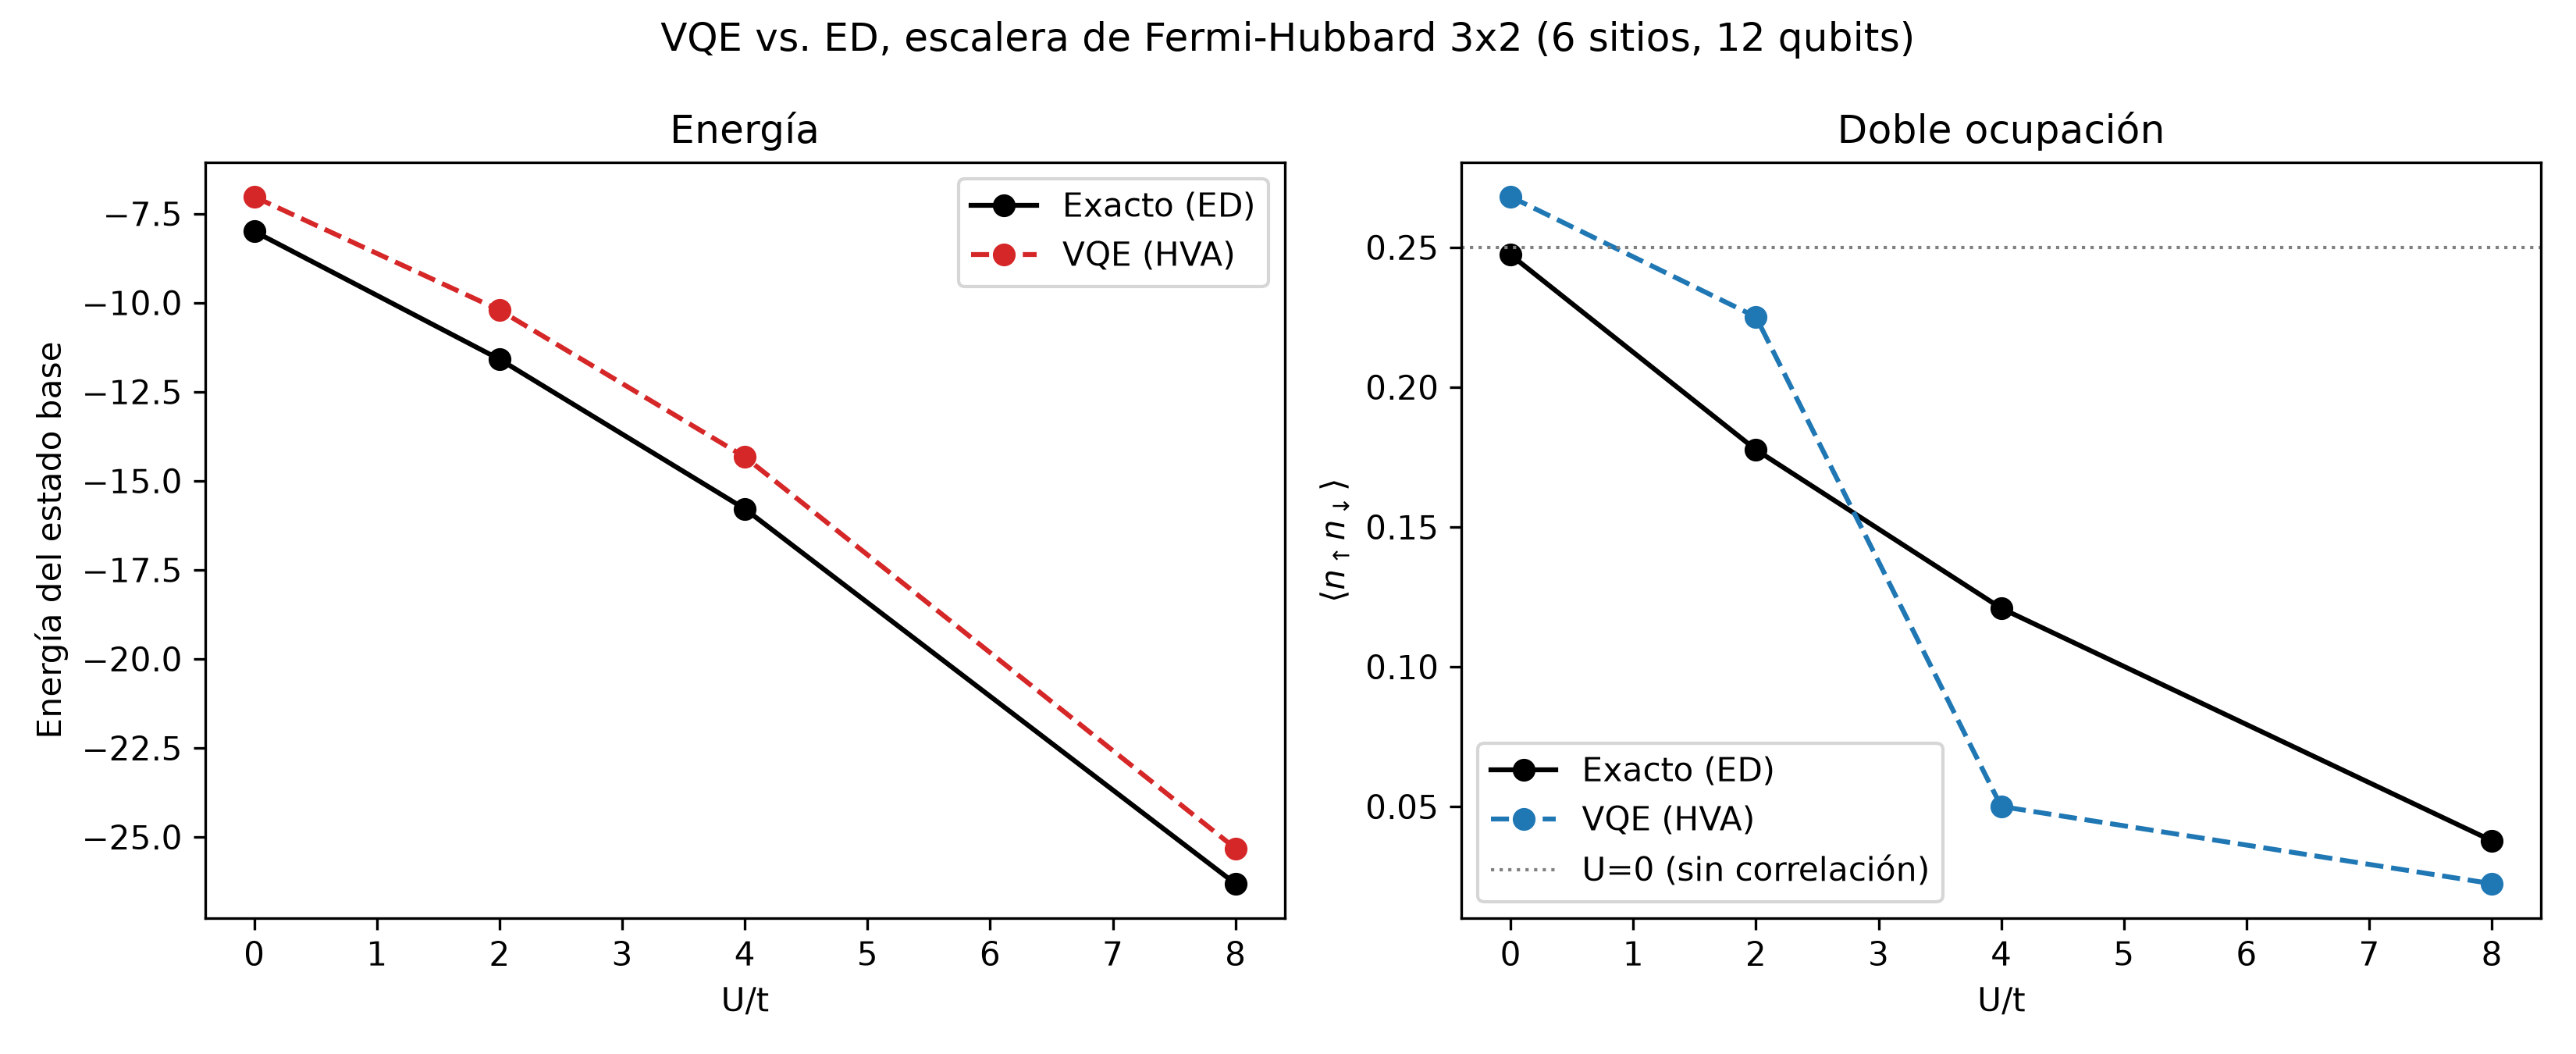
\includegraphics[width=\textwidth]{../fermi_hubbard_vqe_vs_ed.png}
    \end{column}
    \begin{column}{0.42\textwidth}
      \small
      \begin{itemize}
        \item Mismas compuertas que Trotter, con \textbf{48 ángulos libres}; conserva
          $N_\uparrow,N_\downarrow$ por construcción.
        \item COBYLA, 3 reinicios $\times$ 600 iteraciones.
        \item \good{Tendencia correcta.}
        \item \warn{Brecha en energía de $\sim$+1} (4--12\,\%) en todo el barrido.
        \item \warn{Doble ocupación inconsistente:} $0.225$ vs.\ $0.178$ ($U{=}2$);
          $0.050$ vs.\ $0.121$ ($U{=}4$).
      \end{itemize}
    \end{column}
  \end{columns}
  \vspace{0.3em}
  \centering\small El cuello de botella es el \textbf{optimizador}, no el Hamiltoniano (se
  verificó contra ED).
\end{frame}

% ============================================================= 8:45 -- 10:00
\begin{frame}{Conclusiones}
  \begin{enumerate}
    \item \good{Trotter reproduce la dinámica exacta} dentro del ruido de shots y captura física
      real: la supresión del decaimiento de doblones a $U$ grande.
    \item \good{El error de Trotter está controlado y medido}: converge con pendiente $\approx2$
      en dos redes distintas.
    \item \warn{VQE es el cuello de botella}: capta la tendencia, no la precisión, y su costo
      decidió el tamaño de todo el proyecto.
    \item \warn{A 6 sitios, el tamaño finito domina}: estado base triplete hasta
      $U/t\approx4.3$; la física de singlete de peldaño aparece solo después.
  \end{enumerate}
  \vspace{0.4em}
  \begin{block}{Siguientes pasos}
    Gradientes por \emph{parameter-shift} para VQE \;·\; Trotter de segundo orden (Suzuki)
    \;·\; redes más grandes con \emph{fermionic SWAP} \;·\; hardware real con ruido.
  \end{block}
  \vfill
  \centering \large \textcolor{qDeep}{\textbf{Gracias -- preguntas}}
\end{frame}

\end{document}
